%%%%%%%%%%%%%%%%%%%%%%%%%%%%%%%%%%%%%%%%%%%%%%%%%%%%%%%%%%%%%%%%%%%%%%%%%%%%%%%
%
% results
% Copyright (c) 2010 by tilo.mueller@rwth-aachen.de
% 
%%%%%%%%%%%%%%%%%%%%%%%%%%%%%%%%%%%%%%%%%%%%%%%%%%%%%%%%%%%%%%%%%%%%%%%%%%%%%%%

\chapter{Ergebnisse}

TODO: Roadmap (erst am Ende, "Kapitel 4 unterteilt sich in ... Unterkapitel und ...)

\section{Demographie}
\label{sec:demo}
Die Studiendurchführung ergab 1020 beantwortet Fragebögen. Nach bereinigung der Daten sind hieraus 856 vollständig bewertbare Fragebögen hervorgekommen.
Von den 856 Teilnehmern waren 204 (23,8\%) weiblich, 613 (71,6\%) männlich und 39 haben keine Angabe zu ihrem Geschlecht abgegeben. Die hohe Anzahl an männlichen Teilnehmern liegt vermutlich daran, dass die Umfrage über den Email-Verteiler der Technischen Fakultät der Universität Erlangen-Nürnberg verteilt wurde, welche einen höheren Männer- als Frauenanteil hat.
Im Mittelwert waren die Teilnehner 25,0 Jahre alt, mit einer Standardabweichung von 9,2 Jahren.
Interessant ist, dass trotz des niedrigen Wertes und der geringen Standardabweichung dennoch einige Fragebögen im Altersbereich von 45 bis 77 liegen. Dies wir in der weiteren Ausarbeitung gesondert betrachtet - denn selbst wenn ihre Anzahl nicht für statistisch exakte Aussagen reicht könnten hier dennoch interessante Ergebnisse gefunden werden.
Beim höchsten erreichten Bildungsabschluss zeigt sich dass ein Großteil der Teilnehmer entweder gerade studiert oder bereits einen Abschluss im Studium erreicht hat. Abitur und Bachelor/Master/Diplom zusammen geben über 90\% der Teilnehmer ab. Nur knapp über 5,7\% der Befragten hatten einen Haupt- oder Realschulabschluss.
Somit spiegelt die demographische Verteilung der Studienteilnehmer nicht die Gesamtzahl der Google-Nutzer in Deutschland wieder, da schon 2001 17,9\% der Deutschen mit Volks-/Hauptschulabschluss das Internet genutzt haben (nach Grafik "Nutzeranteil nach Bevölkerungsgruppen" \cite{ard2001internetusage}). In einer zukünftigen Arbeit zu diesem Thema sollten eventuell speziell die Gruppen "Kein Abschluss", "Hauptschulabschluss" und "Realschulabschluss" betrachtet werden.

\begin{figure}[H]
\centering
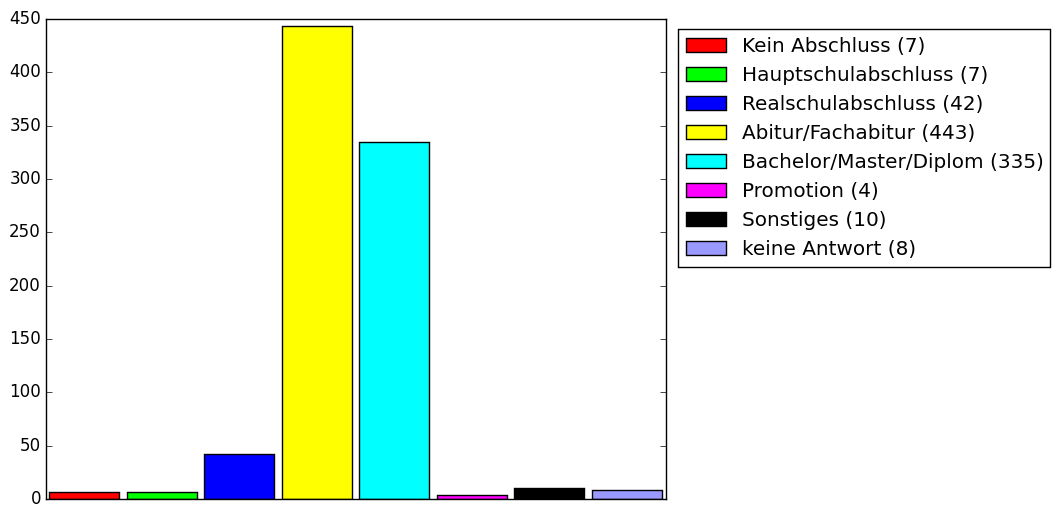
\includegraphics[scale=0.55]{images/schulabschluss}\\
\caption{Höchster Schulabschluss}\label{schulabschluss}
\end{figure}
Auch die Auswertungen zu der derzeitigen Arbeitsbeschäftigung zeigen ein ähnliches Bild - 77,0\% der Teilnehmer (659) waren zum Zeitpunkt der Studiendurchführung Studenten. Dahingegen sind nur 2,0\% in Ausbildung und 15,0\% berufstätig.
Das arithmetische Mittel der selbst eingeschätzten Informatikkenntnisse liegt auf einer Skala von 1 (keine) bis 5 (sehr hohe) bei 3,3. Hier wurde angenommen, dass im Durchschnitt ein Wert von 3,0 erreicht wird, da dies der Mittelwert der auszuwählenden Optionen war und man bei spezialisiertem Wissen von einer homogenen Verteilung ausgehen kann. Dass dieser Wert sehr nah an dem von mir erwartetem Mittelwert von 3,0 liegt deutet darauf hin, dass die Umfrage trotz der geringen Anzahl an Realschülern und Hauptschülern dennoch Relevanz hat, wenn man weiterhin annimmt, dass der Wissenstand im Bereich Informatik hier der ausschlaggebende Faktor ist und nicht der Bildungsstand.
Diese Statistik verschiebt sich stark, wenn man die Frage nach den Kenntnissen in der IT-Sicherheit betrachtet. Hier liegt das arithmetische Mittel bei 2,6, was um 0,6 niedriger ist als das arithmetische Mittel der IT Kenntnisse.\\
Die weiteren demographischen Ergebnisse sind der Übersichtlichkeit halber in Tabelle \ref{demoqna} zusammengefasst.\\
%TODO: Korellation - Kein Bildungsabschluss in der Informatik bedeuted geringeres Wissen in IT Security: 77,5\% der Teilnehmer haben keinen Bildungsabschluss in der Informatik oder einem anderen IT-nahem Fachbereich.
%Grafisch darstellen: steigende Funktion (Excel Tabelle, Pivottabelle, Youtube, Berechnung signifikant)

\begin{table}
	\begin{tabular}[]{ l | l | c | c }
	\hline
	Frage & Antwort & Anzahl (absolut) & Anzahl (relativ) \\
	\hline
	& weiblich &  204 & 23,8\% \\
	Sind Sie:& männlich & 613 & 71,6\% \\
	& keine Antwort & 39 & 4,6\% \\
	\hline \hline
	& Kein Abschluss & 7 & 0,8\% \\
	& Hauptschulabschluss & 7 & 0,8\% \\
	& Realschulabschluss & 42 & 4,9\% \\
	Welchen höchsten Schulablschluss& Abitur/Fachabitur & 443 & 51,75\% \\
	haben Sie? & Bachelor/Master/Diplom & 335 & 39,1\% \\
	& Promotion & 4 & 0,5\% \\
	& Sonstiges & 10 & 1,2\% \\
	& keine Antwort & 8 & 1,0\% \\
	\hline \hline
	& In Ausbildung & 17 & 2,0\% \\
	& Student/-in & 659 & 77,0\% \\
	& Berufstätig & 127 & 15,0\%\\
	Sie sind derzeit: & In Rente & 4 & 0,5\% \\
	& Nicht Berufstätig & 19 & 2,2\% \\
	& Sonstiges & 23 & 2,7\% \\
	& keine Antwort & 7 & 0,8\% \\
	\hline \hline
	& 1 & 23 & 2,7\%\\
	& 2 & 205 & 24,2\% \\
	Wie hoch schätzen Sie ihre & 3 & 266 & 31,4\% \\
	Informatik Kenntnisse ein? & 4 & 239 & 28,2\% \\
	& 5 & 114 & 13,5\% \\
	& keine Antwort & 9 & 1,0\% \\
	\hline \hline
	& 1 & 143 & 16,8\% \\
	& 2 & 262 & 31,0\% \\
	Haben Sie Kenntnisse im& 3 & 253 & 29,8\% \\
	Bereich IT-Sicherheit?& 4 & 151 & 17,8\% \\
	& 5 & 40 & 4,7\% \\
	& keine Antwort & 7 & 0,8\% \\
	\hline \hline
	Haben Sie einen Bildungsabschluss & Ja & 184 & 21,5\% \\
	in der Informatik oder einem anderen & Nein & 663 & 77,5\%\\
	IT-nahem Fachbereich? & keine Antwort & 9 & 1,0\% \\
	\hline
	\end{tabular}
	\caption{Demographische Fragen und Ergebnisse}\label{demoqna}
\end{table}

\section{Hypothesen}
Bei Betrachtung der Kategorie, in der es sich um die Nutzung der Google Dienste handelt, fällt sofort auf, dass diese sehr aktiv genutzt werden. Auf "Wie aktiv nutzen Sie die folgenden Dienste? Google Suche:" antworteten fast 90\% mit 4 und 5, davon sind 73,7\% bei der 5 angesiedelt. Auch nutzen über die Hälfte der Umfrageteilnehmer (58,9\%) Android mit einer Aktivität von 4 oder 5.
Die Dienste die tatsächlich zu Google gehören wurden von einem großem Anteil der Teilnehmer auch Google zugeordnet. Android, Picasa, Google+, Hangouts, Gmail, Youtube und Chrome wurden je von mehr als 50\% der Teilnehmern Google zugeordnet. Dabei ist die Zugehörigkeit von Picasa zu Google mit 51,2\% am unbekanntesten, Google+ und Gmail sind mit 97,6\% und 92,4\% am öftesten angewählt worden. Die Dienste die nicht zu Google gehören wurden auch zum Großteil nicht zugeordnet, den größten Wert hat Whatsapp mit 6,4\%, was ein sehr geringer Wert ist.\\
Die Mehrheit der Teilnehmer (64,7\%) besitzt einen Google Account, 2 oder mehr Accounts besitzt werden von 21,7\%.\\
Auch das Wissen der Umfrageteilnehmer zu Google ist zum Großteil gut. So wissen 85,9\% der Teilnehmer, dass Google auf Nutzer zugeschnittene Werbung anbietet und nur 3,0\% sind der Meinung, dass Google dies nicht tut. Ein ähnliches Bild zeigt sich bei der Frage nach den auf Nutzer zugeschnittenen Suchergebnissen. Hier sind mit 81,0\% der Teilnehmer zwar ein bisschen weniger der Meinung, dass Google dies anbietet, aber eine Rate von über 80\% ist immernoch sehr hoch (siehe Tabelle \ref{fittingAdsAndSearch}).\\
\begin{table}
	\begin{tabular}[]{l| l | c | c}
		\hline
		Fage & Antwort & Anzahl (absolut) & Anzahl (relativ)\\ \hline \hline
		Bietet Google auf Nutzer& Ja & 735 & 85,9\%\\
		zugeschnittene Werbung an? & Nein & 26 & 3,0\%\\
		& Weiß nicht & 95 & 11,1\% \\
		\hline
		Bietet Google auf Nutzer& Ja & 693 & 81,0\% \\
		zugeschnittene Suchergebnisse an? & Nein & 40 & 4,7\% \\
		& Weiß nicht & 123 & 14,4\% \\
		 \hline
	\end{tabular}
	\caption{Anbieten von zugeschnittener Werbung und Suchergebnissen von Seiten Googles}\label{fittingAdsAndSearch}
\end{table}
\\"Meine Daten sind bei Google sicher" und "Durch die Nutzung von Google Diensten gebe ich zu viel von meiner Privatsphäre auf" korrelieren nur relativ schwach mit r(854) = -0.29 und einer zweiseitigen Signifikanz von nahezu 0,00. Es ergibt sich also eine indirekte Korrelation, die allerdings nur sehr schwach ist. Eine leichte Tendenz ist dennoch vorhanden.

\section{Forschungsfragen}

\section{Sonstiges}
